\documentclass{article}
\usepackage{parskip}
\usepackage{listings}
\usepackage{pdfpages}
\usepackage[margin=.6in]{geometry}
\begin{document}
\includepdf[pages=4]{Module4.pdf}
\includepdf[pages=5]{Module4.pdf}
Its nearly impossible to predict all of the hops a packet will make through the internet before it gets to its destination.

\includepdf[pages=6]{Module4.pdf}
At first internet was just local so no one attempted to attack over it. Because of this most network protocols didn't really have any security concerns in mind.

The link layer is most of the local stuff (things on your home system) and the network layer is where IP (internet protocol) comes in. It is the connections between networks. The transport layer determines which application gets your information. The main protocols for this are TCP (transmission control protocol) and UDP (user datagram protocol). Choosing between these is a design choice. TCP is more reliable but UDP is faster. The application layer is where you see stuff like ssl and http and such.

All of you information is divided into packets allowing you to encapsulate each layer. 
\begin{itemize}
	\item Ethernet Header
	\item IP header
	\item TCP/UDP header
	\item HTTP application layer - also called the payload
\end{itemize}

\includepdf[pages=8]{Module4.pdf}
A server can have multiple applications running on it. These are distinguished by ports. The server has a table (called port allocation table) that maps port numbers to processes. A port scan is used to gain information. Attempt to open a connection on every port to know what kinds of software is running on the machine.

\begin{tabular}{|c|c|}
\textbf{port} & \textbf{pid}\\
21 & ftp\\
22 & ssh\\
80 & http\\
\end{tabular}

Some webservers will straight up tell you what kind of server it is. Apache tells you not only that it is an Apache server, but tells you the exact version its running.

\includepdf[pages=9]{Module4.pdf}
Applications that give away too much information is \textbf{loose-lipped}. You can see if there are known vulnerabilities in this software if you know what kind is being used and what version. Vulnerability databases store all this information and some will even provide scripts that will break into a server for you (commonly used by script kiddies).

NMAP is a tool that sends packets to all possible ips on the network and sees if it gets a response. Once you have a list of machines on the network you can port scan them to see what they are running. 

\includepdf[pages=10]{Module4.pdf}
This attack had a slightly different response of you are or are not an valid user. From this you can find out if someone has an account with them

\includepdf[pages=11]{Module4.pdf}
There is a search engine called Shodan that searches for devices connected to the internet. Github is also bad for letting you find people that put code in their public repo that contains passwords.

\includepdf[pages=12]{Module4.pdf}
Its usually safe to assume that you are being listened to. 

\includepdf[pages=13]{Module4.pdf}
Copper cable is very noisy so its pretty easy to listen over it without even altering the cable. You can get these things that just clamp onto the cable and listen to it without altering it at all. Cat5 don't work as well because there are lots of cables wound around eachother.

Optical fiber is a lot harder. If you bend the cable a bit some light escapes that can be listened to. The US got caught with a submarine that bends under water cables to listen to them.

Wireless communication (like microwaves and satallite) can be intercepted because the area that gets the beam to hit it is very large (beam is cone shaped). 

\includepdf[pages=14]{Module4.pdf}
Wifi is super easy to monitor. There are distributions of linux that can turn your laptop into a monitoring device. The range is actually pretty good (up to kilometers away in good conditions, current record is 180km).

People might not just want to eavesdrop on you, they might be wanting to use your resources (like stealing wifi).

\includepdf[pages=15]{Module4.pdf}
Some things get sent to a destination that they shouldn't (like hitting reply to all). Switches are used to send packets to people over time. Say Alice sends stuff to Bob, if the switch has not seen Bob it doesn't know where to send it so it sends it to everyone and sees if Bob replies saying where he is. This is an instance of people getting shit they shouldn't.

\includepdf[pages=16]{Module4.pdf}
Once you can impersonate someone it because super easy to handle stuff. 

\includepdf[pages=17]{Module4.pdf}
Spoofing is basically saying you are something that you arent. Closely related to phishing attacks. An evil twin attack on wifi access points is basically making you router look like another one (the config is basically free range). You can even change the mac address, so there is nothing that forces them to be unique so that you can make them identical even if you connect to something automatically. 

\includepdf[pages=18]{Module4.pdf}
This is basically taking over a session that is in progress by overriding values in the session to make yourself look like an endpoint. You can do this through cookies (yay).

A facebook example: when you log in facebook creates a session id that it stores in a cookie and returns to you so that when you try to access things you send the session id and knows who you are and what you have access to. The only part that goes over https is the login and session id return. When you request knew pages and send the session id it was unsecure so people eavesdropping could get the session id from the request. Now they store that in a cookie on their broswer and facebook will now believe that they are that person.

Someone make a firefox plugin called firesheep that you could run while sitting on a public network. It would grab all the session ids that went through and allowed you to log in as those people.

\includepdf[pages=19]{Module4.pdf}
This is looking and patterns in the data being sent to make guesses about what is being sent. For instance we can tell if you are downloading a movie because there will be multiple connections going on, but not if you are just looking at a page its fine.

\includepdf[pages=20]{Module4.pdf}
This is where people modify packets while they are being transmitted. The security against this is the TCP checksum. Its not at all hard for the attacker to just update the checksum so its not really that great of a defense.

\includepdf[pages=21]{Module4.pdf}
When we look stuff up we need to look up the address associated with the url, but an attacker can change the value returned from the lookup to make an incorrect mapping. A solution is proposed called DNSSEC (look more into it).

\includepdf[pages=22]{Module4.pdf}
Theres lots of holes in this because it was formulated at a time when people trusted everyone on the network. There is also programmer error and shit. 

\includepdf[pages=23]{Module4.pdf}

\includepdf[pages=24]{Module4.pdf}
Theres lots of ways that attackers can get at web servers (usually through the url). For example it was usually common to be able to enter \texttt{example.com/../../../etc/password} and actually get the example. A way to to fix this would be to run it in a chroot jail.

Windows servers would allow you to run executables with command line arguments through the same url hacking. 

\includepdf[pages=25]{Module4.pdf}
Cross-site scripting(XSS) and request forgery(CSRF) allow people to inject code.

XSS - say we have a vulnerable website, the attacker adds in a script tag that gets content from the attackers server and executes it, so that when the user contacts the site all of the content gets sent to them and that script gets executed.

CSRF - works like XSS but instead of loading in a script it references a url that does some action

Defenses
\begin{itemize}
	\item don't use urls that execute things, always require it to be a post
	\item don't allow the site to reference external scripts
\end{itemize}
As with all things there are ways around the defense.

\includepdf[pages=26]{Module4.pdf}
Send a bunch of requests to something causing it to go down because it cannot respond because its too busy processing all of these requests. A \textbf{ping flood} is sending a ton of pings causing a DoS. Its easy to spot lots of requests from the same source and just ignore them to get around it. So you can \textbf{smurf} your attack by impersonating someone else (forge the from address). 

\includepdf[pages=27]{Module4.pdf}
Send a SYN packet with some special flags and then the server sends an ACK (acknowledgement) packet and you must send an ACK packet back to acknowledge you got the acknowledgement. An attacker can leverage this by sending a ton of SYNs (causes an entry for each one to added in memory) but they never send the ACK response to finish the connection. Eventually this table fills up and new people cannot connects. This is called a \textbf{syn flood}.

If we send a very large packet it will fragment up. An attacker can send packets labeled such that it looks like theres a missing packet (like sending 1, 2, and 4). The server cannot do anything about these packets until the final one arrives so they just sit there eating up memory.
E
A router broadcasts to the network that they are there and who they are connected to. Theres tons of communications going on all the time. Nothing stops the routers from lying about what they are and what they are connected to. For example Pakistan wanted to censor out youtube. To do this they created a cheap path that said it was to youtube but actually went to a different router that would just drop the packets. This accidentally got out to china telling the whole internet that there was a cheaper path to youtube which censored youtube to the whole world. Google fixed this by making the distance to the real youtube much cheaper. (cheapness is actually just how specific the address range is) 

\includepdf[pages=28]{Module4.pdf}

\includepdf[pages=29]{Module4.pdf}

\includepdf[pages=30]{Module4.pdf}
Basically these are just bot nets. All bots connect to a server run by the attacker and ask if there is a command that needs to be run. Frequently there is a suicide command that will uninstall the bot software. 

\includepdf[pages=31]{Module4.pdf}
Amplification is when you find servers that respond with very large amounts of data, you send them a request and spoof the source address to be the thing you want to attack. An example is an attack on Spamhaus (creates black lists that isp can block) with around 300 Gb/s. This overwhelmed an exchanged making it so that accessing a lot of european sites was very slow. Another attack used the NTP protocol to amplify up to 400 Gb/s to someplaces in isreal. Supposidly there was a DoS that got up to 500 Gb/s setting the record.

\includepdf[pages=32]{Module4.pdf}

\includepdf[pages=33]{Module4.pdf}
Botnets want to be as stealthy as possible so that you don't remove them.

\includepdf[pages=34]{Module4.pdf}
Most bot net have software updates the distribute. Some do fast flux where they pass around who will be the command node. Domain generation algorithms allow the bots in the net generate a list of potential domain names and keeps checking which of them is the command node so that people trying to take down the network has a harder time tracking down where the control node is. Conficker was one of the biggest bot nets ever, resulting in the Conficker Working Group continuously figuring out the list of generated domain names and blocking access to them. This results in the bots not getting any commands. 

\includepdf[pages=35]{Module4.pdf}

\includepdf[pages=36]{Module4.pdf}

\includepdf[pages=37]{Module4.pdf}

\includepdf[pages=38]{Module4.pdf}

\includepdf[pages=39]{Module4.pdf}

\includepdf[pages=40]{Module4.pdf}

\includepdf[pages=41]{Module4.pdf}

\includepdf[pages=42]{Module4.pdf}

\includepdf[pages=43]{Module4.pdf}

\includepdf[pages=44]{Module4.pdf}

\includepdf[pages=45]{Module4.pdf}

\includepdf[pages=46]{Module4.pdf}

\includepdf[pages=47]{Module4.pdf}

\includepdf[pages=48]{Module4.pdf}

\includepdf[pages=49]{Module4.pdf}

\includepdf[pages=50]{Module4.pdf}

\includepdf[pages=51]{Module4.pdf}

\includepdf[pages=52]{Module4.pdf}
\includepdf[pages=53]{Module4.pdf}
Personal firewalls are different than dedicated machines (put them between the world and the server) as these run on your machine. Most of these will forbid everything and then ask you for permission. This is done so that you can see when something malicious is trying to access the internet. 

\includepdf[pages=54]{Module4.pdf}
Can also prevent attacks on servers that are running on your computer. For instance running a dev server on your machine that you don't want anyone accessing. Windows XP had a bunch of servers running on it before the first patch that had a ton of vulnerabilities. 

\includepdf[pages=55]{Module4.pdf}
We have somethings that we don't want to be super protected (some people should be able to access it). So we create and demilitarized zone and we let packets through the external firewall through to that zone.

\includepdf[pages=57]{Module4.pdf}
You set up a trap for an attacker. You can register an email account but never use for anything so that any email you get there has been brute forced and will thus be spammed. So you can add that email to spam list. Similarly you can create a server that does nothing and ping anyone that accesses it because they shouldn't be looking for it. Some researchers use honey pot networks to let attackers do their thing in a safe space. From this they can see what attacks are being run without getting fucked. Attackers might figure out that they are in a honey pot so they stop what they are doing (same as with sandboxes or VMs). 

Be careful that you dont accidentally put the honey pot behind the dmz or other not safe places.

\includepdf[pages=58]{Module4.pdf}
Low interaction means that they are easy to run. A common one is honeyd which has a bunch of vulnerable software on it. There are some kiddie scripts that check if they are running in honeyd. 

A high interaction requires way more setup. 

\includepdf[pages=60]{Module4.pdf}
Sometimes we try to define what is normal behavior and anyone acting outside that gets an alarm raised.

\includepdf[pages=61]{Module4.pdf}
Host based run on a machine. Problem is you can only see the network traffic coming to your machine and not elsewhere. Another problem is that if someone gets access to your machine so they can get rid of the IDS.

Network based run on a dedicated machine. This means that they are very hard to attack because they can only run just the IDS and are often not even connected to the network.  

Its not uncommon to use a combination of multiple kinds of IDS in a distributed system.

\includepdf[pages=62]{Module4.pdf}
We know a bunch of heuristics to spot common attacks. These are hard coded rules where we can see if behavior matches them. These are really easy for the attacker to get around. 

\includepdf[pages=63]{Module4.pdf}
These create much more general definitions of good behavior and flag behavior outside that. This often works via scoring (where bad behavior builds the score) and once some threshold is reached stuff get triggered. This is to prevent a bunch of false positives. There is a learning phase when you first set this up so that it can figure out what good behavior is. 

\includepdf[pages=64]{Module4.pdf}
There are some free IDSs that you can play with, a network based one called Bro and host based one called Snort.

A very specific example is Tripwire. It is anomoly based, host based IDS. It watches for an attacker modifying files that you normally wouldn't. To do this is creates a digital fingerprint of each system file (usually a hash of it) and export them to some place the attacker cannot get to. When the attacker gets into the systems and does something that changes a system file the hash for the file is no long the same which is a warning.

We want to make sure that we are calculating the hashes of a file not on the production machine because a rootkit might alter how your machine views or hashes files. So you should pull the hard drive or run a different os.

\includepdf[pages=65]{Module4.pdf}














\end{document}